\chapter{Creating a Sphere using Gmsh}
\thispagestyle{empty}
\label{sec:chap17}
\newcommand{\LocCHonesevenfig}{\Origin/CHAPTERS/chap17/figures}

In the earlier chapter we learnt about how to Install and Run Gmsh by creating a simple geometry. As the earlier tutorial shows about basic geometry construction in Gmsh the user is expected to know it before starting this chapter. This chapter deals with creating a Sphere using Gmsh and meshing it. The chapter we will focus on creating the spherical geometry and the domain surrounding it and in the next chapter we will look into how to mesh this geometry. Since this is a spherical geometry we will learn about how to create a circular arc, how to create ruled surface and doing basic manipulation with the .geo file which generated. 

\section{Points}

You can start Gmsh by either double clicking on the gmsh-icon or from the terminal by typing \textbf{gmsh sphere1.geo} , this will open up the gmsh window. The first step after starting Gmsh is to mark the co-ordinates for our sphere, we define the center of the Sphere and points surrounding it. Co-ordinates for the sphere ( 7 points ) are as given below : \newline

\begin{itemize}

\item (0, 0, 0)
\item (-1, 0, 0)
\item (1, 0, 0)
\item (0, -1, 0)
\item (0, 1, 0)
\item (0, 0, -1)
\item (0, 0, 1)

\end{itemize}

\flushleft The points will appear on the Gmsh window as shown in the Fig \ref{points} below.

\begin{figure}[h]  
\centering
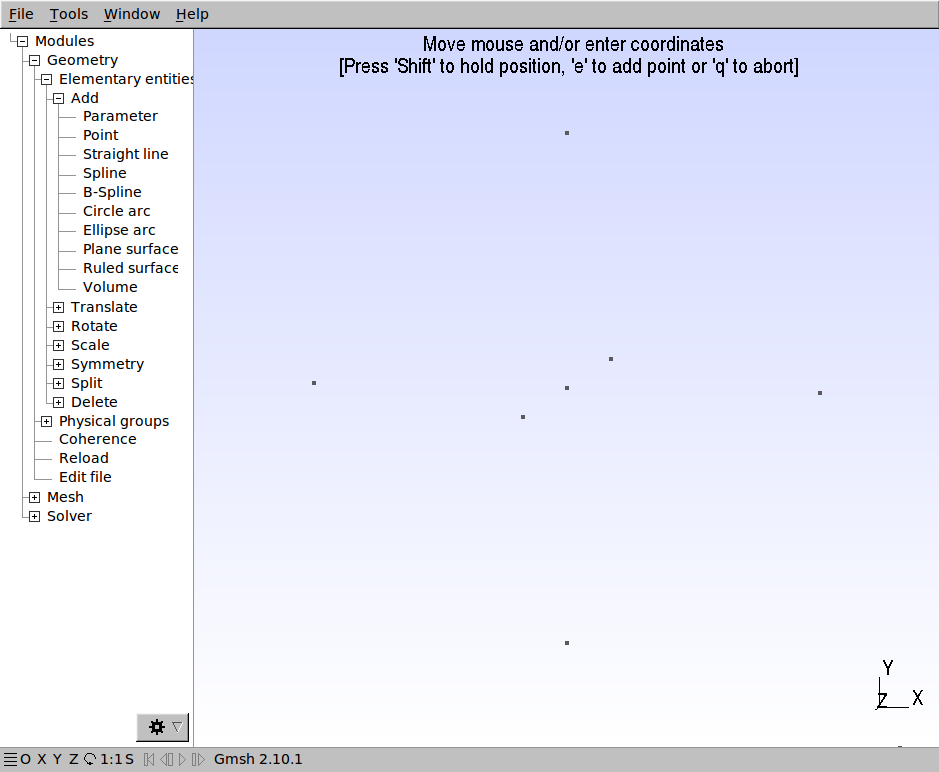
\includegraphics[scale=0.25]{\LocCHonesevenfig/gmshpts.png}
\caption{Sphere coordinates}
\label{points}
\end{figure}

\section{Circular Arc}

Creating an Arc is a three step process where we a start point, center and an end point . An important point to be noted here is that in Gmsh a Circular Arc is strictly created less than pi. Now to create an circular arc select Circle Arc option in the left hand side menu of Gmsh under Add. Click on the right most point in the Gmsh Window, it will turn red in colour, Fig \ref {point1}.

\begin{figure}[h]  
\centering
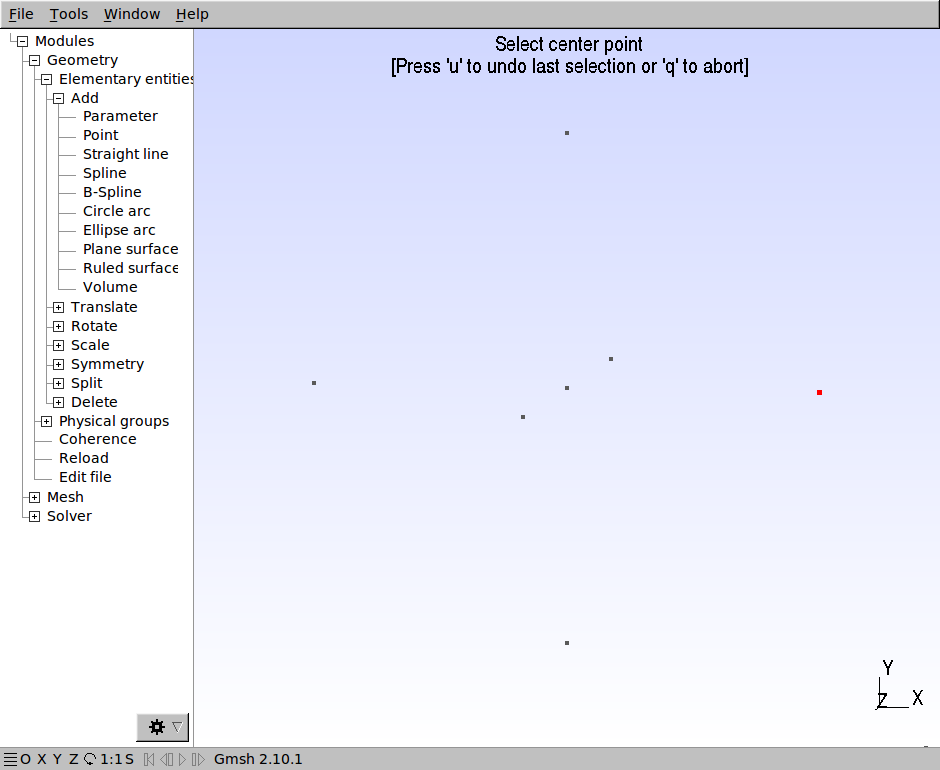
\includegraphics[scale=0.25]{\LocCHonesevenfig/point1.png}
\caption{Rightmost point}
\label{point1}
\end{figure}

\flushleft Now click on the center of the Sphere as shown in Fig \ref{point2} and that too will turn red in colour.

\begin{figure}[h]  
\centering
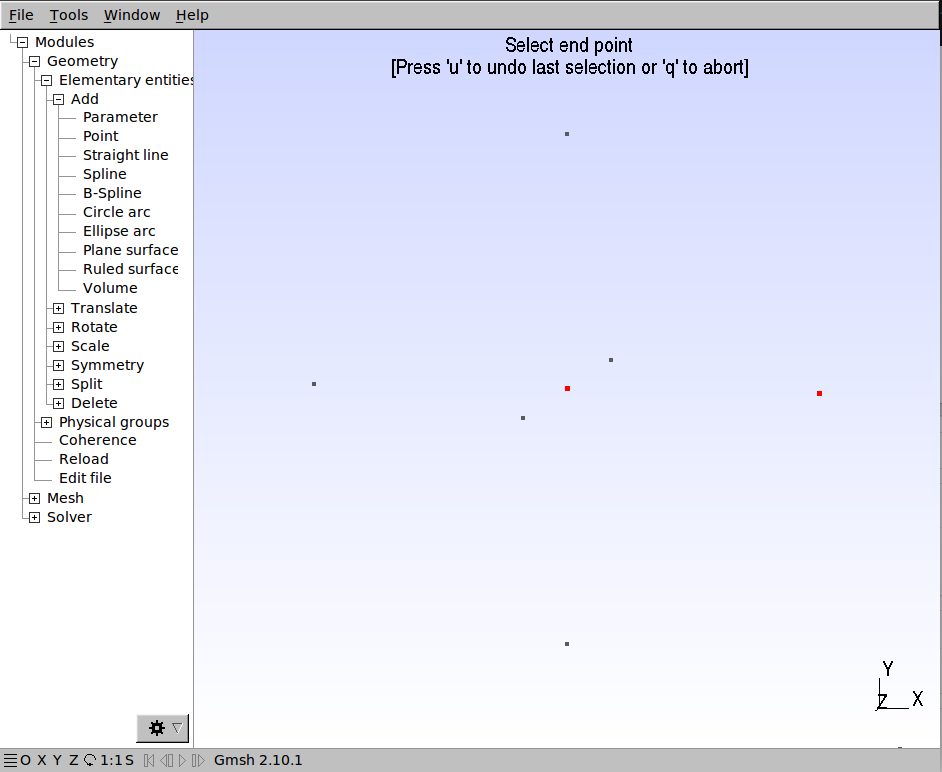
\includegraphics[scale=0.25]{\LocCHonesevenfig/point2.png}
\caption{Center of the sphere}
\label{point2}
\end{figure}

\flushleft For the end point click on the point above the center. As soon as we click on this point a arc is created as shown in the Fig \ref{point3}.

\begin{figure}[h]  
\centering
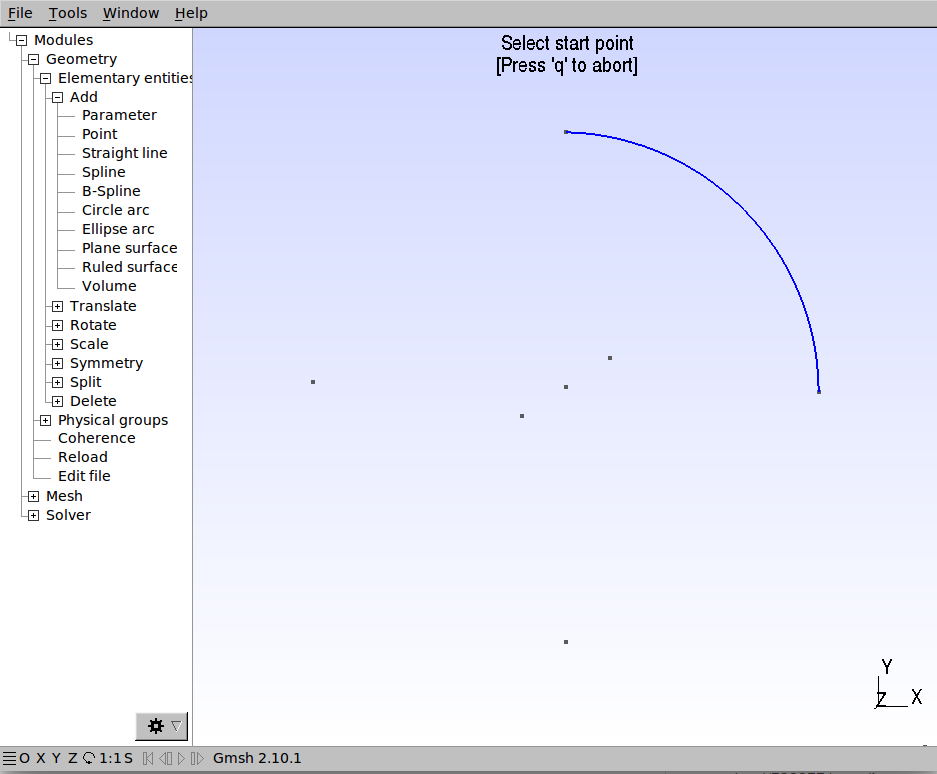
\includegraphics[scale=0.25]{\LocCHonesevenfig/point3.png}
\caption{End point of the Arc}
\label{point3}
\end{figure}

\flushleft Repeat this process for all the points to complete the sphere. Create the Arcs keeping the same center point. The completed geometry of the sphere is as shown , Fig \ref{}

\begin{figure}[h]  
\centering
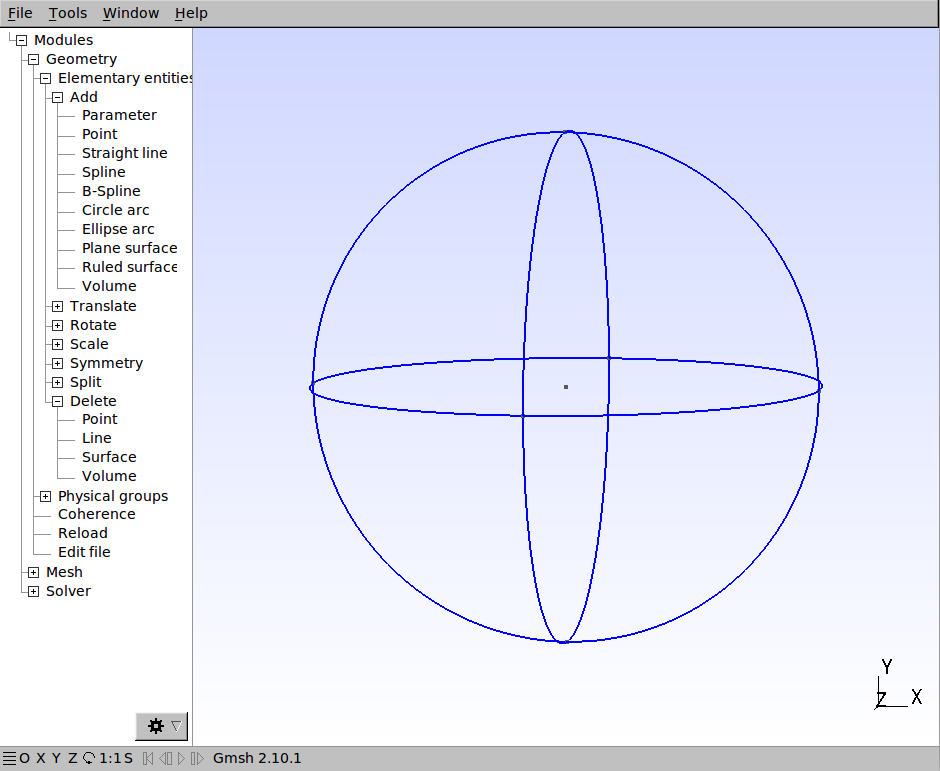
\includegraphics[scale=0.25]{\LocCHonesevenfig/sphere.png}
\caption{Sphere}
\label{sphere}
\end{figure}

\section{Surface Creation}

To stich the arcs together we now need to create surfaces. To do so, click on the Ruled Surface option under Add menu. Now select bounding edges for the surface as shown in Fig \ref{surface}. After the selction they will turn red in colour. Press e on your keyboard to execute this selection. A crossed dotted line will be visible which shows that the surface has been created, Fig \ref{surf1}. Repeat the process to create all eight surfaces of the sphere, Fig \ref{surf2}.

\begin{figure}[h]  
\centering
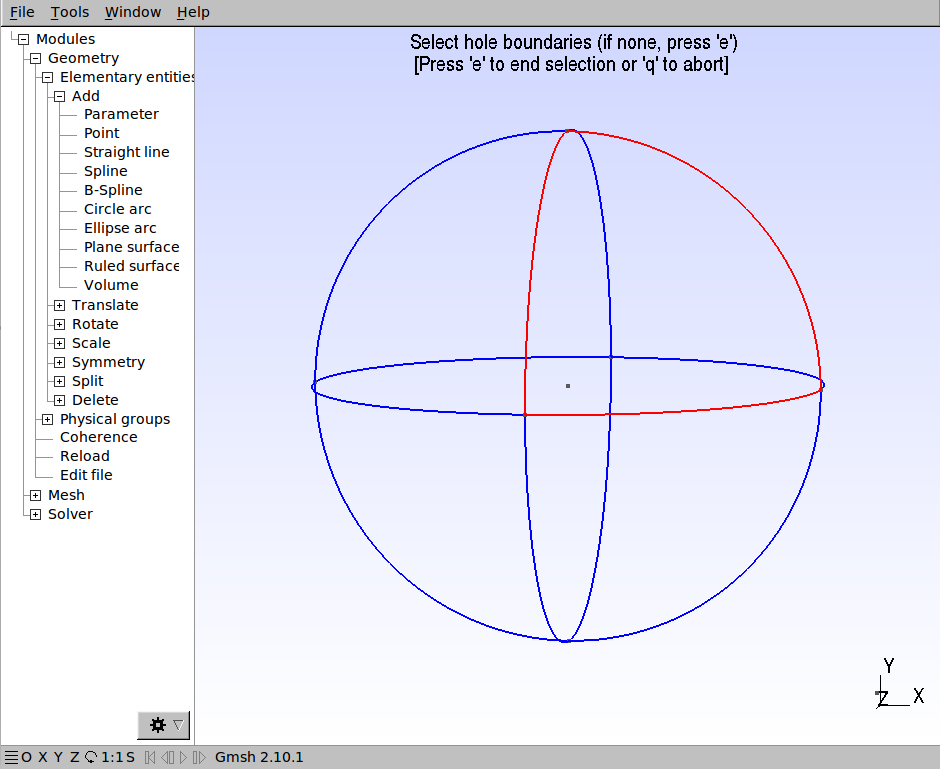
\includegraphics[scale=0.25]{\LocCHonesevenfig/surface.png}
\caption{Surface Bounding edges}
\label{surface}
\end{figure}

\begin{figure}[h]  
\centering
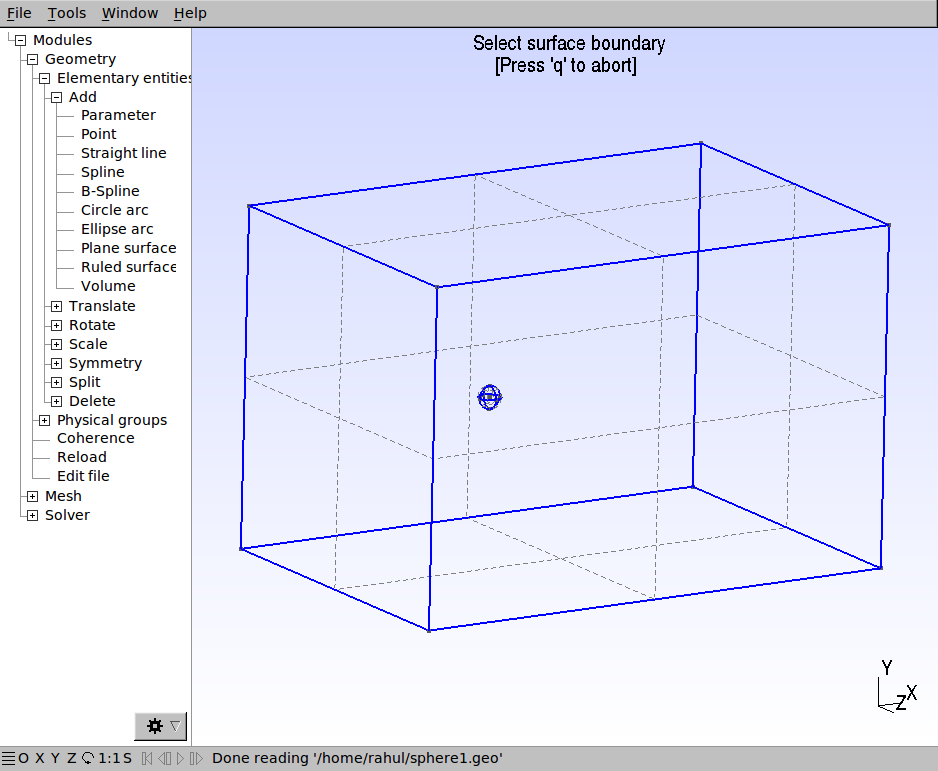
\includegraphics[scale=0.25]{\LocCHonesevenfig/surf1.png}
\caption{Surface Creation}
\label{surf1}
\end{figure}

\begin{figure}[h]  
\centering
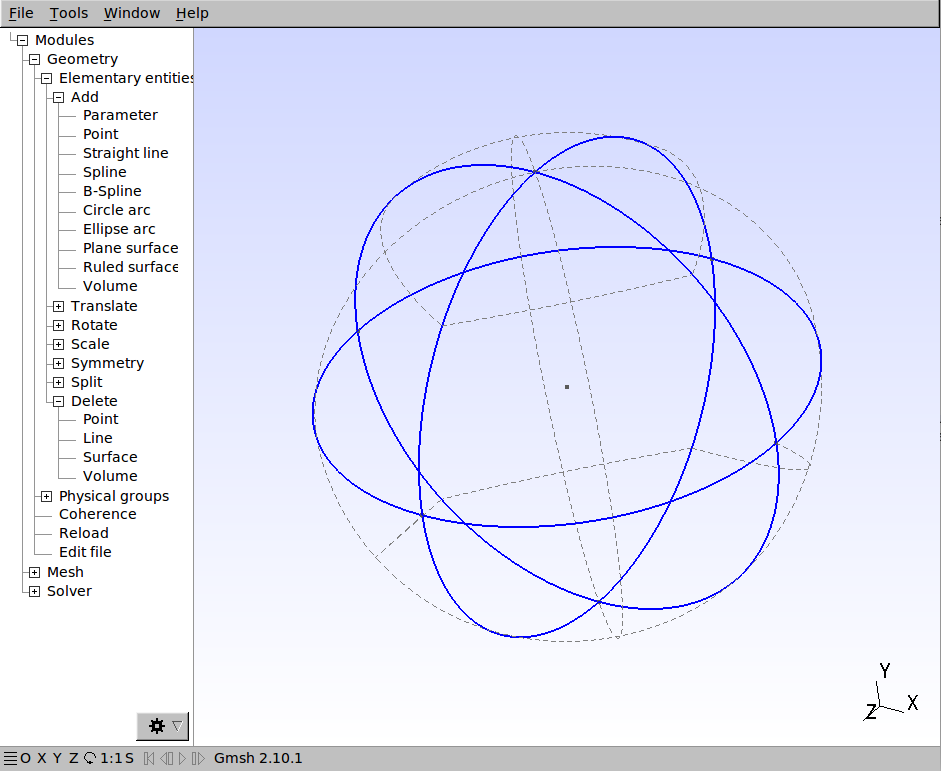
\includegraphics[scale=0.25]{\LocCHonesevenfig/surf2.png}
\caption{Complete Surface Creation}
\label{surf2}
\end{figure}

\section{Editing .geo file}

Gmsh provides us with an option of editing the saved file. Open sphere1.geo file in any editor of your choice. Information related to the geometric entities we create using Gmsh are stored here. General syntax under gmsh is as given below,\newline

\centering Point (1) = {0,0,0,1}; \newline

\flushleft here Point stand for the Geometrical Entity, (1) stands for Identification number inside the parenthesis next number starting from one which is equal to an expression. For points in expression we have the X, Y and Z co-ordinate followed by the value of desired mesh element size. The size of the mesh element will then be computed by linearly interpolating these values on initial mesh. We can change the mesh element size here by a variable which can then take different value. Change the mesh element size from 1 to s and on top of the file type s = 0.1; as shown in the Fig \ref{var}

\begin{figure}[h]  
\centering
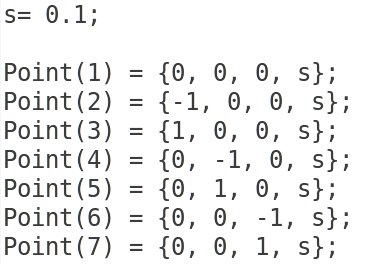
\includegraphics[scale=0.35]{\LocCHonesevenfig/var.png}
\caption{Mesh Element size variable}
\label{var}
\end{figure}

\section{Boundary Layer}

Flow over any bluff body we are more interested in capturing the Boundary Layer. In this problem to capture the boundary layer in the geo file add a line after the mesh characteristic length varialble as \newline

\centering  \textbf{Mesh.CharacteristicLengthFromCurvature = 0.05;} \\

\flushleft This line above will adapt the mesh to the curvature w.r.t the geometrical entities.

\section{Volume Creation}

To create a volume we need all the bounding surfaces. This can also be done manually by typing at the end of the file \newline

\centering \textbf{Surface Loop (identity) = {identities of sphere surface within braces};} \\

\flushleft Now save this file and close it

\section{Physical Groups}

The geometry created now needs a physical meaning to it which helps us during simulation. To do this under Physical Groups go to Surface and select all the 8 surfaces of the sphere. It will turn red in colour, Fig \ref{surf4}. Press e to end selction and q to abort. Now again open the sphere1.geo file. It can be noticed that a new line has been added to the file which describes the physical surface. Here replace the Identification number by the name sphere within double quotes as this can be used as a boundary identification during simulation or postprocessing.\newline

\centering \textbf{Physical Surface("Sphere") = {26, 27, 28, 30, 31, 32, 33, 34};} \\

\flushleft Save and close the file. 

\begin{figure}[h]  
\centering
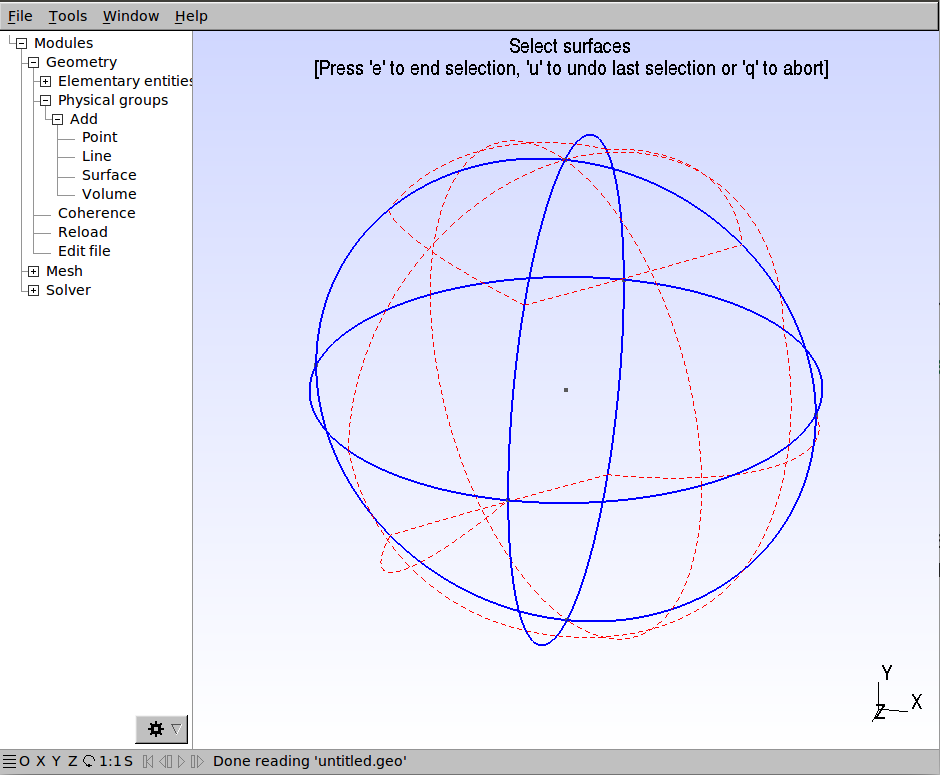
\includegraphics[scale=0.25]{\LocCHonesevenfig/surf4.png}
\caption{Physical Groups : Surface}
\label{surf4}
\end{figure}
 


